\documentclass[t,aspectratio=169,xcolor=dvipsnames]{beamer}
\usetheme{SimplePlusAIC}

\usepackage{graphicx}
\usepackage{booktabs}
\usepackage{svg}
\usepackage{tcolorbox}
\usepackage{tikz}
\usetikzlibrary{shapes.geometric, arrows, positioning, fit, calc}
\usepackage{makecell}
\usepackage{listings}

\newcommand*{\defeq}{\stackrel{\text{def}}{=}}
\usepackage{setspace}
\usepackage[T1]{fontenc}
\usepackage{helvet}
\usepackage{amsmath}
\usepackage{ragged2e}
\usepackage{gensymb}

\usepackage[svgnames,table]{xcolor}
\arrayrulecolor{black}
\setlength{\arrayrulewidth}{0.20mm}
\renewcommand{\arraystretch}{1.35}

% Highlight istilah penting: bold + merah
\newcommand{\tem}[1]{\textbf{\textcolor{red}{#1}}}

% Konfigurasi listings (jika ada kode)
\lstset{
    basicstyle=\ttfamily\small,
    breaklines=true,
    columns=fullflexible,
    frame=none
}

\title[File System Dasar]{File System Dasar \& Disk Scheduling}
\subtitle{Week 12: Konsep File, Direktori, Inode, dan Disk Scheduling}
\author[informatika-itera.github.io/os]{informatika-itera.github.io/os}
\institute[ITERA]{Program Studi Teknik Informatika \\ Institut Teknologi Sumatera}
\date{\textcolor{nyublue}{2026}}

\AtBeginSection[]{
    \begin{frame}[plain]
        \vfill
        \centering
        {\usebeamerfont{title}\color{nyublue}\Large \insertsectionhead\par}
        \vspace{0.3cm}
        {\large Week 12}
        \vfill
    \end{frame}
}

\begin{document}

% 1. Title frame
\begin{frame}
    \titlepage
\end{frame}

% 2. Outline frame
\begin{frame}
    \frametitle{Outline}
    \tableofcontents
\end{frame}

% 3. Capaian Pembelajaran
\begin{frame}
    \frametitle{Capaian Pembelajaran}
    \framesubtitle{Tujuan setelah pertemuan selesai}
    \small
    \begin{enumerate}
        \item Menjelaskan konsep persistence dan urgensinya dalam sistem operasi.
        \item Menggambarkan abstraksi file dan direktori beserta analoginya.
        \item Memahami apa itu inode dan perannya dalam file system.
        \item Menganalisis masalah dan solusi terkait \textit{disk scheduling} (FCFS, SSTF, SCAN, C-SCAN).
    \end{enumerate}
    \vspace{0.5cm}
    \begin{exampleblock}{Fokus Kelas Ini}
        Kita fokus pada \tem{konsep Persistence}, \tem{File System}, dan \tem{Disk Scheduling}.
    \end{exampleblock}
\end{frame}

%================================================
% BAGIAN 1: PERSISTENCE & ABSTRAKSI
%================================================
\section{Konsep Persistence \& Abstraksi File}

\begin{frame}[plain]
    \begin{center}
        \vspace{3cm}
        \Huge\textbf{Konsep Persistence \& Abstraksi File}
    \end{center}
\end{frame}

%--- Slide 1: Masalah Volatilitas ---
\begin{frame}[shrink=5]
    \frametitle{Masalah: RAM itu Pelupa}
    \framesubtitle{Data hilang saat listrik mati atau program selesai}

    \begin{columns}[T]
        \column{0.48\textwidth}
        \begin{alertblock}{Masalah Volatilitas}
            \begin{itemize}
                \item Memori utama (RAM) bersifat \tem{volatile}.
                \item Semua data, perhitungan, dan \textit{state} proses hilang saat:
                \begin{itemize}
                    \item Komputer dimatikan/crash.
                    \item Program (proses) selesai jalan.
                \end{itemize}
            \end{itemize}
        \end{alertblock}

        \column{0.48\textwidth}
        \begin{exampleblock}{Kebutuhan Kita}
            Kita butuh menyimpan data hasil kerja (dokumen, foto, kode) agar tetap ada esok hari.
            Kebutuhan ini menuntut ruang penyimpanan yang besar, tahan lama, dan aman.
        \end{exampleblock}
    \end{columns}
\end{frame}

%--- Slide 2: Analogi ---
\begin{frame}
    \frametitle{Analogi: Meja Kerja vs Lemari Arsip}
    \framesubtitle{Mengapa kita butuh dua jenis tempat penyimpanan}

    \begin{columns}[T]
        \column{0.48\textwidth}
        \begin{block}{RAM = Meja Kerja}
            \begin{itemize}
                \item Sangat dekat dan cepat dijangkau.
                \item Kapasitas terbatas.
                \item Di akhir hari (dimatikan), meja harus dibersihkan total.
            \end{itemize}
        \end{block}

        \column{0.48\textwidth}
        \begin{block}{Storage = Lemari Arsip Baja}
            \begin{itemize}
                \item Sedikit lebih jauh dan lambat.
                \item Kapasitas luar biasa besar.
                \item Data \tem{aman dan permanen} meskipun kantor sedang tutup.
            \end{itemize}
        \end{block}
    \end{columns}

    \vspace{0.4cm}
    \begin{exampleblock}{Tugas Sistem Operasi}
        OS bertugas memindahkan data dari "meja kerja" ke dalam "lemari arsip" secara rapi, agar mudah dicari lagi besok.
    \end{exampleblock}
\end{frame}

%--- Slide 3: Persistence ---
\begin{frame}
    \frametitle{Konsep Persistence (Ketahanan Data)}
    \framesubtitle{Menjaga data tetap hidup melampaui proses yang membuatnya}
    \small

    \begin{columns}[T]
        \column{0.50\textwidth}
        \textbf{Apa itu Persistence?}
        \begin{itemize}
            \item Kemampuan sistem mempertahankan \textit{state} (data) meskipun listrik terputus.
            \item Menggunakan \textit{hardware} khusus: \textit{Hard Disk Drive} (HDD) atau \textit{Solid State Drive} (SSD).
        \end{itemize}
        
        \column{0.46\textwidth}
        \textbf{Tantangan OS:}
        \begin{itemize}
            \item Disk fisik hanyalah deretan panjang sektor-sektor mentah (biasanya 512 bytes).
            \item Bagaimana cara pengguna membedakan "foto liburan" dengan "tugas OS" di disk yang sama?
        \end{itemize}
    \end{columns}

    \vspace{0.4cm}
    \begin{alertblock}{Solusi: Abstraksi}
        OS tidak membiarkan pengguna membaca disk per sektor. OS menciptakan abstraksi yang mudah dipahami: \tem{File} dan \tem{Direktori}.
    \end{alertblock}
\end{frame}

%--- Slide 4: Abstraksi File ---
\begin{frame}
    \frametitle{Abstraksi Pertama: File}
    \framesubtitle{Hanya sekumpulan byte dengan nama}
    \small

    \begin{columns}[T]
        \column{0.48\textwidth}
        \begin{block}{Apa itu File?}
            File adalah abstraksi OS untuk kumpulan data yang saling terkait. Bagi OS, file hanyalah sebuah \tem{\textit{array of bytes}} linier.
        \end{block}

        \begin{itemize}
            \item Setiap file punya \textbf{nama tingkat tinggi} (\texttt{tugas.pdf}).
            \item OS yang bertugas memetakan nama file ini ke blok/sektor fisik di dalam disk.
        \end{itemize}

        \column{0.48\textwidth}
        \begin{exampleblock}{Nomor Inode}
            Di sistem UNIX/Linux, di bawah layar, setiap file sebenarnya diidentifikasi dengan nomor unik yang disebut \tem{\textit{inode number}}. OS mengubah nama file menjadi nomor ini.
        \end{exampleblock}
    \end{columns}
\end{frame}

%--- Slide 5: Operasi Dasar File ---
\begin{frame}[fragile]
    \frametitle{Mekanisme Interaksi dengan File}
    \framesubtitle{Sistem operasi menyediakan API standar untuk membaca/menulis}
    \footnotesize

    \begin{columns}[T]
        \column{0.54\textwidth}
\begin{lstlisting}[basicstyle=\ttfamily\scriptsize]
// 1. Buka/buat file
int fd = open("tugas.txt", O_CREAT | O_WRONLY);

// 2. Tulis data
write(fd, "Halo dunia", 10);

// 3. Sinkronisasi (opsional)
fsync(fd);

// 4. Tutup
close(fd);
\end{lstlisting}

        \column{0.42\textwidth}
        \begin{block}{API File}
            \begin{enumerate}
                \item \texttt{open()}: Minta izin OS, dapat \textit{file descriptor}.
                \item \texttt{read() / write()}: Pindahkan data.
                \item \texttt{fsync()}: Paksa data turun dari cache RAM langsung ke disk fisik.
                \item \texttt{close()}: Lepas sumber daya.
            \end{enumerate}
        \end{block}
    \end{columns}
\end{frame}

%--- Slide 6: Abstraksi Direktori ---
\begin{frame}
    \frametitle{Abstraksi Kedua: Direktori}
    \framesubtitle{Agar ribuan file tidak berserakan}
    \small

    \begin{columns}[T]
        \column{0.48\textwidth}
        \begin{block}{Apa itu Direktori?}
            Secara teknis, direktori hanyalah \tem{file khusus} yang berisi daftar pasangan: \\
            \texttt{(Nama File $\to$ Nomor Inode)}
        \end{block}
        
        \begin{itemize}
            \item Karena direktori bisa menyimpan direktori lain, terbentuklah struktur \tem{hierarki (\textit{tree})}.
            \item Berawal dari satu \textit{root} (\texttt{/}).
        \end{itemize}

        \column{0.48\textwidth}
        \begin{exampleblock}{Analogi}
            File adalah "dokumen" lembaran. Direktori adalah "map" (folder) yang mengelompokkan dokumen-dokumen terkait dalam laci lemari arsip.
        \end{exampleblock}
    \end{columns}
\end{frame}

%================================================
% BAGIAN 2: INODE & METADATA
%================================================
\section{Struktur Internal: Inode \& Metadata}

\begin{frame}[plain]
    \begin{center}
        \vspace{3cm}
        \Huge\textbf{Struktur Internal: Inode \& Metadata}\\[0.4em]
        \Large\textit{Bagaimana OS Menyimpan File di Balik Layar}
    \end{center}
\end{frame}

%--- Slide 1: Konsep Inode ---
\begin{frame}[shrink=5]
    \frametitle{Apa itu Inode (\textit{Index Node})?}
    \framesubtitle{Pemisahan antara nama, metadata, dan data}
    \small

    \begin{columns}[T]
        \column{0.50\textwidth}
        Bagi sistem operasi, file \textbf{bukanlah} namanya.\\
        File direpresentasikan oleh sebuah struktur data bernama \tem{Inode}.
        \vspace{0.3cm}

        \textbf{Tiga elemen utama file:}
        \begin{enumerate}
            \item \textbf{Nama}: Disimpan di Direktori.
            \item \textbf{Metadata}: Disimpan di Inode.
            \item \textbf{Isi}: Disimpan di \textit{Data Blocks} (Disk).
        \end{enumerate}

        \column{0.48\textwidth}
        \centering
        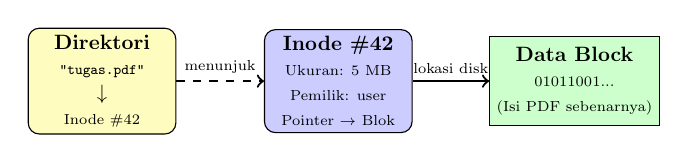
\begin{tikzpicture}[scale=0.75, transform shape]
            % Direktori
            \node[draw, fill=yellow!25, rounded corners, minimum width=2.5cm, minimum height=1.5cm, align=center] (dir) at (0, 0) {\textbf{Direktori}\\\scriptsize \texttt{"tugas.pdf"}\\$\downarrow$\\\scriptsize Inode \#42};
            
            % Inode
            \node[draw, fill=blue!20, rounded corners, minimum width=2.5cm, minimum height=1.5cm, align=center] (inode) at (4, 0) {\textbf{Inode \#42}\\\scriptsize Ukuran: 5 MB\\\scriptsize Pemilik: user\\\scriptsize Pointer $\to$ Blok};
            
            % Data Block
            \node[draw, fill=green!20, minimum width=2.5cm, minimum height=1.5cm, align=center] (data) at (8, 0) {\textbf{Data Block}\\\scriptsize 01011001...\\\scriptsize (Isi PDF sebenarnya)};

            \draw[->, thick, dashed] (dir) -- node[above, font=\scriptsize] {menunjuk} (inode);
            \draw[->, thick] (inode) -- node[above, font=\scriptsize] {lokasi disk} (data);
        \end{tikzpicture}
    \end{columns}
\end{frame}

%--- Slide 2: Analogi Inode ---
\begin{frame}
    \frametitle{Analogi: Perpustakaan Tradisional}
    \framesubtitle{Inode seperti kartu katalog}
    \small

    \begin{columns}[T]
        \column{0.48\textwidth}
        \begin{block}{Kartu Katalog = Inode}
            \begin{itemize}
                \item Berisi informasi: Judul buku, pengarang, tahun terbit, tebal buku.
                \item \textbf{Lokasi fisik}: Rak A, Baris 2.
                \item Kartunya sendiri \tem{bukan buku}, ukurannya kecil dan seragam.
            \end{itemize}
        \end{block}
        
        \column{0.48\textwidth}
        \begin{block}{Buku Fisik = Data Block}
            \begin{itemize}
                \item Buku asli yang tebal dan memakan banyak tempat.
                \item Ada di rak penyimpanan utama (disk fisik).
            \end{itemize}
        \end{block}
    \end{columns}

    \vspace{0.4cm}
    \begin{exampleblock}{Kenapa dipisah?}
        Sangat efisien mencari kartu katalog yang rapi di laci depan daripada harus membongkar seluruh rak gudang hanya untuk mencari siapa pengarang buku.
    \end{exampleblock}
\end{frame}

%--- Slide 3: Melihat Inode (Unix Command) ---
\begin{frame}[fragile]
    \frametitle{Melihat Inode di Terminal}
    \framesubtitle{Menggunakan perintah \texttt{ls -i} dan \texttt{ls -l}}
    \small

    \begin{columns}[T]
        \column{0.55\textwidth}
        \begin{block}{Menampilkan Nomor Inode (\texttt{ls -i})}
\begin{lstlisting}[basicstyle=\ttfamily\scriptsize]
$ ls -i
131093 OS_Slide.pdf
131094 tugas_akhir.docx
\end{lstlisting}
        \end{block}

        \begin{block}{Menampilkan Metadata Dasar (\texttt{ls -l})}
\begin{lstlisting}[basicstyle=\ttfamily\scriptsize]
$ ls -l OS_Slide.pdf
-rw-r--r-- 1 mario users 1048576 May 5 10:00 OS_Slide.pdf
\end{lstlisting}
        \end{block}

        \column{0.42\textwidth}
        \textbf{Apa artinya?}
        \begin{itemize}
            \item \texttt{131093}: Inode number.
            \item \texttt{-rw-r--r--}: Permissions.
            \item \texttt{1}: Jumlah \textit{hard link}.
            \item \texttt{mario users}: Owner \& Group.
            \item \texttt{1048576}: Size (dalam bytes).
            \item \texttt{May 5}: Last modified.
        \end{itemize}
    \end{columns}
\end{frame}

%--- Slide 4: Isi Metadata Lengkap ---
\begin{frame}[fragile,shrink=5]
    \frametitle{Membedah Inode: Perintah \texttt{stat}}
    \framesubtitle{Melihat seluruh metadata yang disimpan oleh OS}
    \small

    \begin{columns}[T]
        \column{0.62\textwidth}
\begin{lstlisting}[basicstyle=\ttfamily\tiny, backgroundcolor=\color{gray!10}]
$ stat OS_Slide.pdf
  File: OS_Slide.pdf
  Size: 1048576       Blocks: 2048       IO Block: 4096   regular file
Device: 802h/2050d    Inode: 131093      Links: 1
Access: (0644/-rw-r--r--)  Uid: ( 1000/   mario)   Gid: ( 100/   users)
Access: 2026-05-05 10:00:00.000000000
Modify: 2026-05-04 15:30:00.000000000
Change: 2026-05-04 15:30:00.000000000
\end{lstlisting}

        \column{0.36\textwidth}
        \begin{alertblock}{3 Jenis Timestamps}
            \begin{itemize}
                \item \tem{Access (atime)}: Kapan file terakhir \textbf{dibaca/dibuka}.
                \item \tem{Modify (mtime)}: Kapan \textbf{isi data} file terakhir diubah.
                \item \tem{Change (ctime)}: Kapan \textbf{metadata} terakhir diubah.
            \end{itemize}
        \end{alertblock}
    \end{columns}
\end{frame}

%--- Slide 5: Pointer di Dalam Inode ---
\begin{frame}[shrink=5]
    \frametitle{Bagaimana Inode Menemukan Data?}
    \framesubtitle{Menggunakan Direct Pointers}
    \small

    Setiap file menempati beberapa blok di disk (misal: blok ukuran 4KB).\\
    Inode menyimpan daftar nomor blok tersebut (\textit{pointers}).

    \vspace{0.3cm}
    \centering
    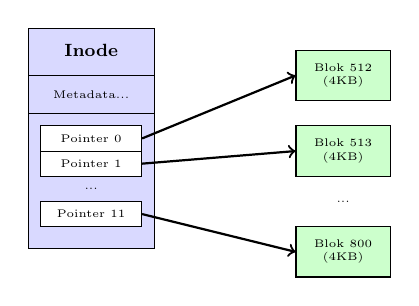
\begin{tikzpicture}[scale=0.8, transform shape]
        % Inode
        \node[draw, fill=blue!15, minimum width=2cm, minimum height=3.5cm, align=center] (inode) at (0,0) {};
        \node[font=\footnotesize\bfseries] at (0, 1.4) {Inode};
        \draw ( -1, 1) -- ( 1, 1);
        \node[font=\tiny] at (0, 0.7) {Metadata...};
        \draw ( -1, 0.4) -- ( 1, 0.4);
        
        % Pointers
        \node[draw, fill=white, minimum width=1.6cm, minimum height=0.4cm, font=\tiny] (p0) at (0, 0) {Pointer 0};
        \node[draw, fill=white, minimum width=1.6cm, minimum height=0.4cm, font=\tiny] (p1) at (0, -0.4) {Pointer 1};
        \node[font=\tiny] at (0, -0.8) {...};
        \node[draw, fill=white, minimum width=1.6cm, minimum height=0.4cm, font=\tiny] (p11) at (0, -1.2) {Pointer 11};

        % Data blocks
        \node[draw, fill=green!20, minimum width=1.5cm, minimum height=0.8cm, font=\tiny, align=center] (d0) at (4, 1) {Blok 512\\(4KB)};
        \node[draw, fill=green!20, minimum width=1.5cm, minimum height=0.8cm, font=\tiny, align=center] (d1) at (4, -0.2) {Blok 513\\(4KB)};
        \node[font=\tiny] at (4, -1) {...};
        \node[draw, fill=green!20, minimum width=1.5cm, minimum height=0.8cm, font=\tiny, align=center] (d11) at (4, -1.8) {Blok 800\\(4KB)};

        % Arrows
        \draw[->, thick] (p0.east) -- (d0.west);
        \draw[->, thick] (p1.east) -- (d1.west);
        \draw[->, thick] (p11.east) -- (d11.west);
    \end{tikzpicture}

    \vspace{0.2cm}
    \begin{block}{Direct Pointers}
        Secara standar, Inode punya 12 pointer langsung. Dengan blok 4KB, ukuran file maksimal hanya: $12 \times 4KB = 48KB$. Bagaimana jika file lebih besar?
    \end{block}
\end{frame}

%--- Slide 6: Indirect Pointers ---
\begin{frame}[shrink=10]
    \frametitle{Menangani File Besar}
    \framesubtitle{Single, Double, dan Triple Indirect Pointers}
    \small

    \begin{columns}[T]
        \column{0.48\textwidth}
        \begin{exampleblock}{Solusi: Blok Indeks}
            OS menggunakan \tem{Indirect Pointer}: pointer di inode \textbf{tidak} menunjuk ke data, melainkan menunjuk ke sebuah blok penuh berisi pointer lain.
        \end{exampleblock}

        \begin{itemize}
            \item \textbf{Single Indirect}: Menunjuk ke blok yang berisi pointer data.
            \item \textbf{Double Indirect}: Menunjuk ke blok yang berisi pointer ke blok \textit{single indirect}.
        \end{itemize}
        Dengan \textit{double/triple indirect}, ukuran file bisa mencapai ukuran Terabytes.

        \column{0.50\textwidth}
        \centering
        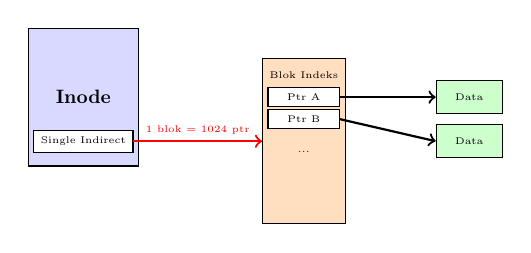
\begin{tikzpicture}[scale=0.7, transform shape]
            \node[draw, fill=blue!15, minimum width=2cm, minimum height=2.5cm, align=center] (inode) at (0,0) {\textbf{Inode}};
            \node[draw, fill=white, minimum width=1.8cm, minimum height=0.4cm, font=\tiny] (p12) at (0, -0.8) {Single Indirect};

            \node[draw, fill=orange!25, minimum width=1.5cm, minimum height=3cm, align=center] (index) at (4,-0.8) {};
            \node[font=\tiny] at (4, 0.4) {Blok Indeks};
            \node[draw, fill=white, minimum width=1.3cm, minimum height=0.3cm, font=\tiny] (ip1) at (4, 0) {Ptr A};
            \node[draw, fill=white, minimum width=1.3cm, minimum height=0.3cm, font=\tiny] (ip2) at (4, -0.4) {Ptr B};
            \node[font=\tiny] at (4, -1) {...};

            \node[draw, fill=green!20, minimum width=1.2cm, minimum height=0.6cm, font=\tiny] (da) at (7, 0) {Data};
            \node[draw, fill=green!20, minimum width=1.2cm, minimum height=0.6cm, font=\tiny] (db) at (7, -0.8) {Data};

            \draw[->, thick, red] (p12.east) -- node[above, font=\tiny]{1 blok = 1024 ptr} (index.west);
            \draw[->, thick] (ip1.east) -- (da.west);
            \draw[->, thick] (ip2.east) -- (db.west);
        \end{tikzpicture}
    \end{columns}
\end{frame}

%--- Slide 7: Hard link vs Soft Link ---
\begin{frame}[fragile,shrink=5]
    \frametitle{Hard Link vs Soft (Symbolic) Link}
    \framesubtitle{Dua cara memberikan nama ganda pada sebuah file}
    \small

    \begin{columns}[T]
        \column{0.48\textwidth}
        \textbf{Hard Link (\texttt{ln})}
        \begin{itemize}
            \item Membuat \textbf{nama baru} di direktori yang menunjuk ke \tem{Inode yang sama}.
            \item Jika file asli dihapus, datanya tetap ada selama masih ada nama lain yang menunjuk (Link count $> 0$).
        \end{itemize}

        \vspace{0.2cm}
        \centering
        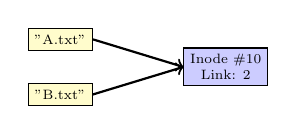
\begin{tikzpicture}[scale=0.7, transform shape]
            \node[draw, fill=yellow!20, font=\scriptsize] (d1) at (0,1) {"A.txt"};
            \node[draw, fill=yellow!20, font=\scriptsize] (d2) at (0,0) {"B.txt"};
            \node[draw, fill=blue!20, font=\scriptsize, align=center] (inode) at (3,0.5) {Inode \#10\\Link: 2};
            
            \draw[->, thick] (d1.east) -- (inode.west);
            \draw[->, thick] (d2.east) -- (inode.west);
        \end{tikzpicture}

        \column{0.48\textwidth}
        \textbf{Soft Link (\texttt{ln -s})}
        \begin{itemize}
            \item Memiliki \tem{Inode sendiri}.
            \item Berisi teks berupa \textit{path} string ke file asli (seperti \textit{shortcut} di Windows).
            \item Jika file asli dihapus, link ini menjadi "mati" (\textit{dangling link}).
        \end{itemize}

        \vspace{0.2cm}
        \centering
        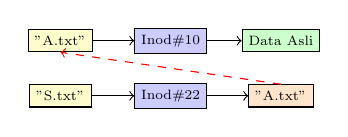
\begin{tikzpicture}[scale=0.7, transform shape]
            \node[draw, fill=yellow!20, font=\scriptsize] (d1) at (0,1) {"A.txt"};
            \node[draw, fill=blue!20, font=\scriptsize] (i1) at (2,1) {Inod\#10};
            \node[draw, fill=green!20, font=\scriptsize] (data) at (4,1) {Data Asli};

            \node[draw, fill=yellow!20, font=\scriptsize] (d2) at (0,0) {"S.txt"};
            \node[draw, fill=blue!20, font=\scriptsize] (i2) at (2,0) {Inod\#22};
            \node[draw, fill=orange!20, font=\scriptsize] (path) at (4,0) {"A.txt"};

            \draw[->] (d1.east) -- (i1.west);
            \draw[->] (i1.east) -- (data.west);
            
            \draw[->] (d2.east) -- (i2.west);
            \draw[->] (i2.east) -- (path.west);
            \draw[->, dashed, red] (path.north) -- (d1.south);
        \end{tikzpicture}
    \end{columns}
\end{frame}

%--- Slide 8: Path Traversal ---
\begin{frame}[shrink=10]
    \frametitle{Path Traversal}
    \framesubtitle{Cara OS mencari \texttt{/home/os.pdf}}
    \small

    Untuk membuka sebuah file, OS harus membaca rentetan direktori dan inode secara bergantian.\\
    OS selalu mulai dari \tem{Root Inode} (biasanya bernomor 2).

    \vspace{0.4cm}
    \centering
    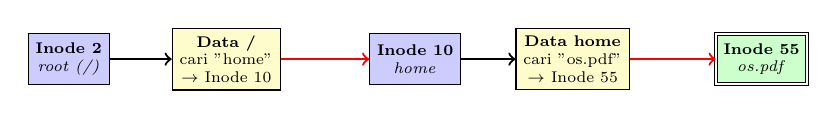
\begin{tikzpicture}[scale=0.8, transform shape]
        % Timeline steps
        \node[draw, fill=blue!20, minimum height=0.8cm, font=\scriptsize, align=center] (r_inode) at (0,0) {\textbf{Inode 2}\\\textit{root (/)}};
        \node[draw, fill=yellow!20, minimum height=0.8cm, font=\scriptsize, align=center] (r_data) at (2.5,0) {\textbf{Data /}\\cari "home"\\$\to$ Inode 10};
        
        \node[draw, fill=blue!20, minimum height=0.8cm, font=\scriptsize, align=center] (h_inode) at (5.5,0) {\textbf{Inode 10}\\\textit{home}};
        \node[draw, fill=yellow!20, minimum height=0.8cm, font=\scriptsize, align=center] (h_data) at (8,0) {\textbf{Data home}\\cari "os.pdf"\\$\to$ Inode 55};

        \node[draw, fill=green!20, minimum height=0.8cm, font=\scriptsize, align=center, double] (f_inode) at (11,0) {\textbf{Inode 55}\\\textit{os.pdf}};

        \draw[->, thick] (r_inode.east) -- (r_data.west);
        \draw[->, thick, red] (r_data.east) -- (h_inode.west);
        \draw[->, thick] (h_inode.east) -- (h_data.west);
        \draw[->, thick, red] (h_data.east) -- (f_inode.west);
    \end{tikzpicture}

    \vspace{0.5cm}
    \begin{alertblock}{Mengapa Membaca File Lambat?}
        Bisa dilihat, sekadar mencari letak `os.pdf` membutuhkan \textbf{banyak operasi I/O ke disk} (baca inode $\to$ baca blok $\to$ baca inode $\to$ dst). Oleh karena itu, OS menggunakan struktur cache di RAM.
    \end{alertblock}
\end{frame}

%--- Slide 9: Checkpoint 2 ---
\begin{frame}
    \frametitle{Checkpoint 2: Inode \& Metadata}
    \framesubtitle{Cek pemahaman sebelum lanjut}
    \small
    \begin{enumerate}
        \item Apa fungsi utama dari Inode?
        \item Perintah Unix apa yang digunakan untuk melihat metadata lengkap (termasuk timestamp) sebuah file?
        \item Jika sebuah file 1 GB menggunakan sistem blok 4KB dan 12 \textit{direct pointers}, bagaimana OS menemukan sisa datanya?
        \item Apa bedanya jika file "Asli.txt" dihapus: ketika kita membuat \textit{Hard Link} vs \textit{Soft Link}?
    \end{enumerate}

    \begin{block}{Kunci Jawaban}
        \scriptsize
        1. Inode menyimpan metadata file (owner, size, permission, timestamps) dan pointer ke blok fisik disk.\\
        2. \texttt{stat [nama\_file]}.\\
        3. OS menggunakan \textit{Indirect Pointers} (blok yang isinya pointer, bukan data).\\
        4. Hard link: file tetap ada, bisa dibaca (link count -1). Soft link: \textit{broken/dangling link}, file tidak bisa dibaca.
    \end{block}
\end{frame}

% 6. Checkpoint
\begin{frame}
    \frametitle{Checkpoint 1: Persistence \& Abstraksi}
    \framesubtitle{Cek pemahaman sebelum lanjut}
    \small
    \begin{enumerate}
        \item Mengapa kita tidak menyimpan semua data secara permanen di RAM saja?
        \item Apa bedanya cara pengguna melihat file vs cara OS melihat file?
        \item Apa isi dari sebuah direktori pada tingkatan teknis terbawah?
    \end{enumerate}
    \vspace{0.5cm}
    \begin{block}{Kunci Jawaban Singkat}
        1. RAM bersifat volatile (hilang saat mati) dan kapasitasnya mahal/terbatas.\\
        2. Pengguna melihat nama file (tingkat tinggi), OS melihat file sebagai \textit{array of bytes} yang dipetakan ke blok fisik disk lewat inode.\\
        3. Daftar pemetaan antara "Nama File" ke "Nomor Inode".
    \end{block}
\end{frame}

% 7. Penutup
\begin{frame}[plain]
    \frametitle{Terima Kasih}
    \begin{center}
        \Huge \textbf{Ada Pertanyaan?}

        \vspace{0.8cm}
        \normalsize
        Sampai jumpa di pertemuan minggu depan!

        \vspace{0.8cm}
        \small
        \textit{``Kutipan inspiratif (opsional).''} \\
        \vspace{0.1cm}
        --- Nama Tokoh
    \end{center}
\end{frame}

\end{document}
